\documentclass[tikz,border=3pt]{standalone}
\usepackage[T1]{fontenc}
\usepackage{lmodern}
\usetikzlibrary{arrows.meta,positioning,fit,backgrounds}
\definecolor{ink}{RGB}{24,39,53}
\definecolor{blue}{RGB}{36,82,126}
\definecolor{pale}{RGB}{239,245,250}
\definecolor{teal}{RGB}{34,108,104}
\definecolor{warm}{RGB}{153,88,42}
\begin{document}

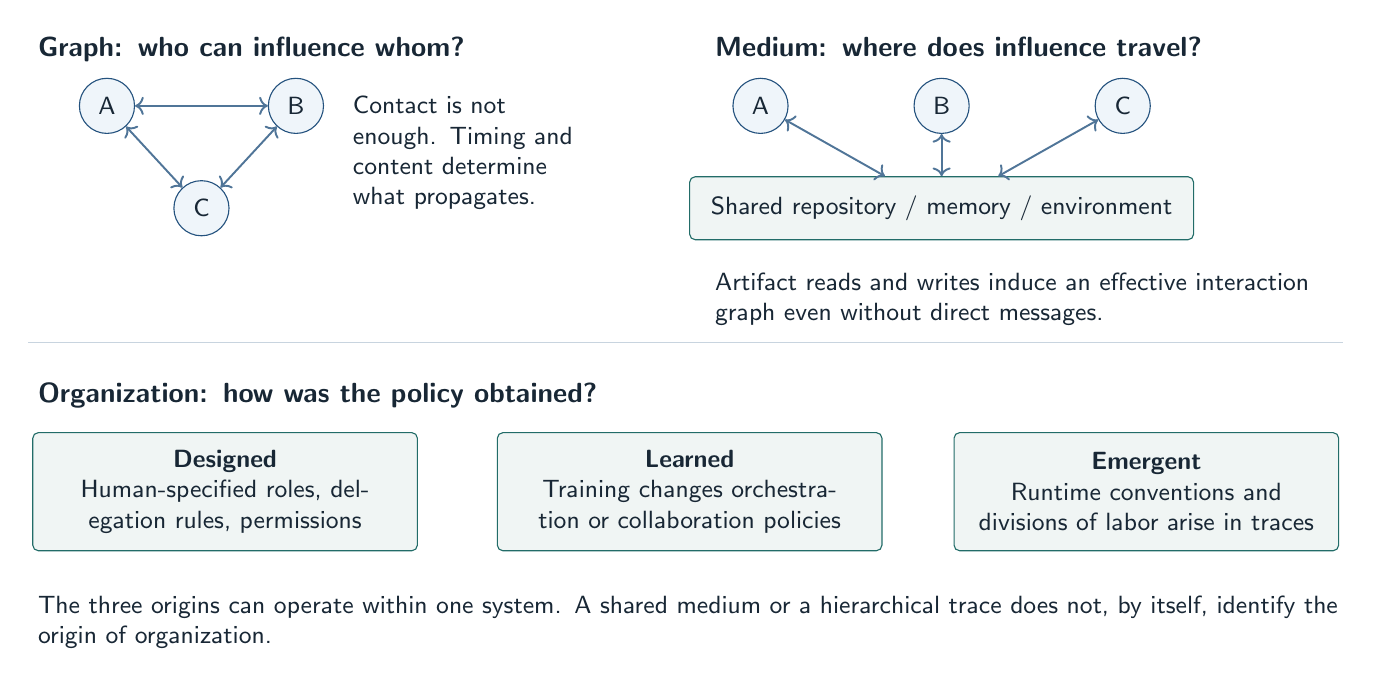
\begin{tikzpicture}[font=\sffamily\small,text=ink,
 agent/.style={circle,draw=blue,fill=pale,minimum size=7mm,inner sep=0pt},
 edge/.style={draw=blue!80,line width=.7pt},
 art/.style={draw=teal,fill=teal!7,rounded corners=2pt,minimum height=8mm,align=center},
 label/.style={align=left,anchor=north west,text width=7.7cm}]
\node[label,font=\sffamily\bfseries] at (0,0) {Graph: who can influence whom?};
\node[agent] (a) at (1.0,-1.0) {A};
\node[agent] (b) at (3.4,-1.0) {B};
\node[agent] (c) at (2.2,-2.3) {C};
\draw[edge,<->] (a)--(b);\draw[edge,<->] (a)--(c);\draw[edge,<->] (b)--(c);
\node[align=left,text width=3cm,anchor=west] at (4,-1.6) {Contact is not enough. Timing and content determine what propagates.};
\node[label,font=\sffamily\bfseries] at (8.6,0) {Medium: where does influence travel?};
\node[agent] (d) at (9.3,-1.0) {A};
\node[agent] (e) at (11.6,-1.0) {B};
\node[agent] (f) at (13.9,-1.0) {C};
\node[art,minimum width=6.4cm] (store) at (11.6,-2.3) {Shared repository / memory / environment};
\draw[edge,<->] (d)--(store);\draw[edge,<->] (e)--(store);\draw[edge,<->] (f)--(store);
\node[label] at (8.6,-3.0) {Artifact reads and writes induce an effective interaction graph even without direct messages.};
\draw[blue!25] (0,-4.0)--(16.7,-4.0);
\node[label,font=\sffamily\bfseries] at (0,-4.4) {Organization: how was the policy obtained?};
\node[art,text width=4.65cm,minimum height=1.5cm] (designed) at (2.5,-5.9)
 {\textbf{Designed}\\Human-specified roles, delegation rules, permissions};
\node[art,text width=4.65cm,minimum height=1.5cm] (learned) at (8.4,-5.9)
 {\textbf{Learned}\\Training changes orchestration or collaboration policies};
\node[art,text width=4.65cm,minimum height=1.5cm] (emergent) at (14.2,-5.9)
 {\textbf{Emergent}\\Runtime conventions and divisions of labor arise in traces};
\node[anchor=north west,align=left,text width=16.7cm] at (0,-7.1)
 {The three origins can operate within one system. A shared medium or a hierarchical trace does not, by itself, identify the origin of organization.};
\end{tikzpicture}
\end{document}
